\documentclass{standalone}
\usepackage{tikz}

\begin{document}
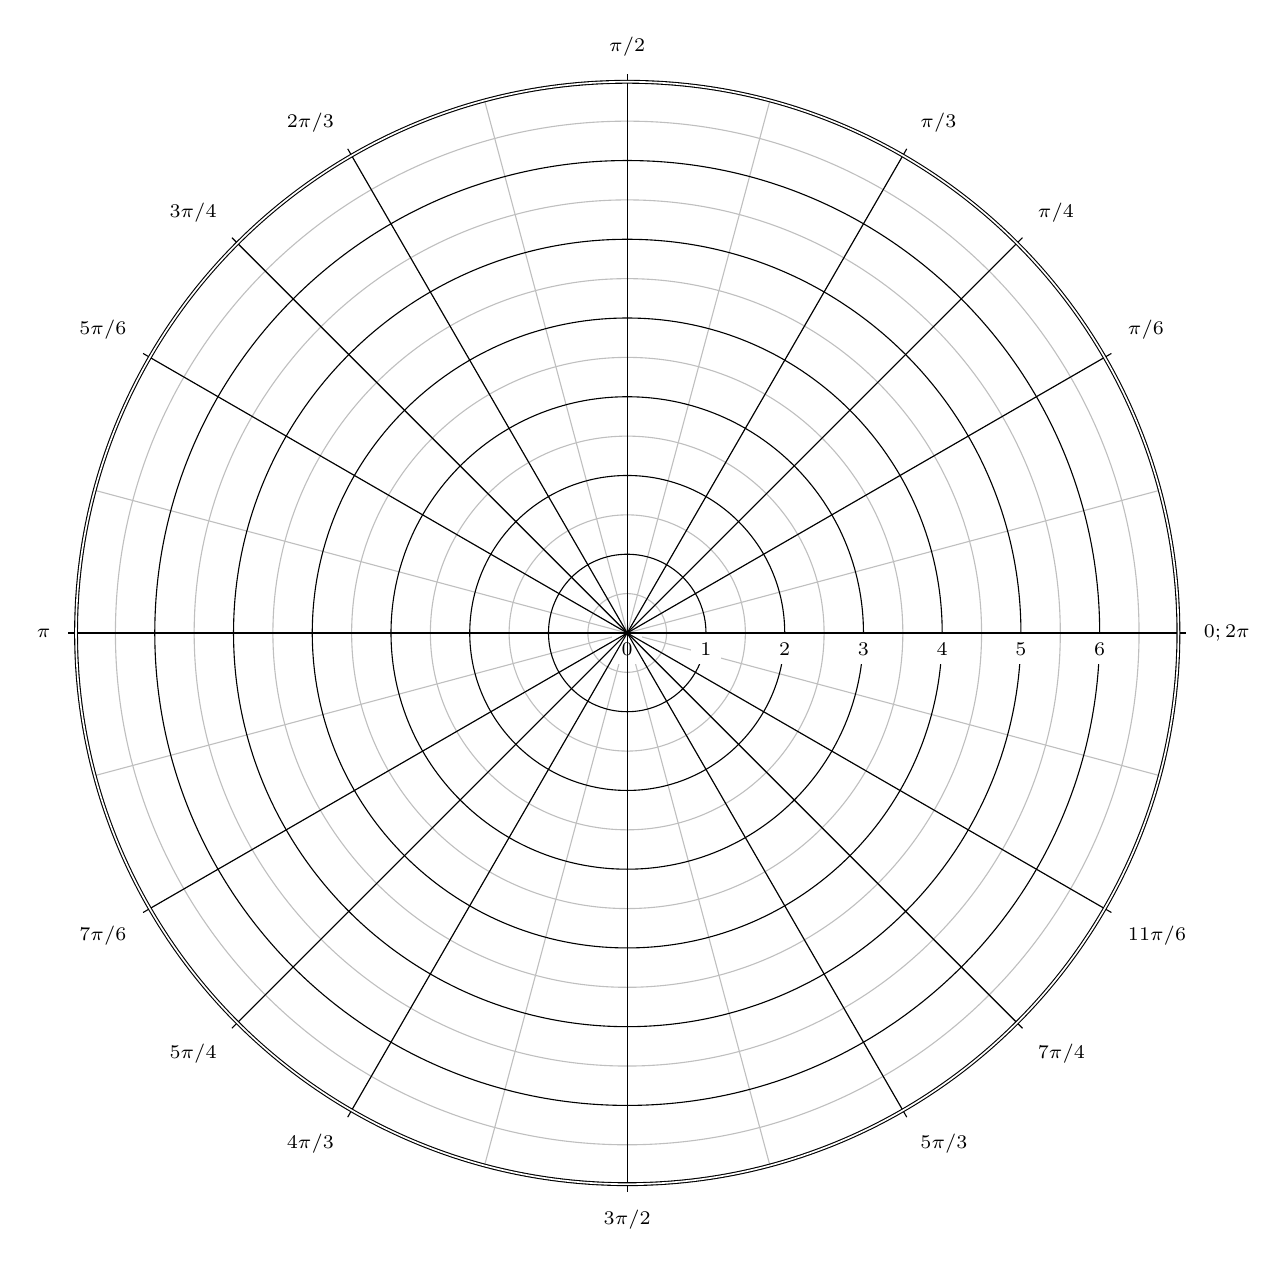
\begin{tikzpicture}[>=latex]

% Draw the lines at multiples of pi/32
\foreach \ang in {0,...,24} {
  \draw [lightgray] (0,0) -- (\ang * 180 / 12:7);
}

% Concentric circles and radius labels
\foreach \s in {0, 1, 2, 3, 4, 5, 6} {
  \draw [lightgray] (0,0) circle (\s + 0.5);
  \draw (0,0) circle (\s);
  \node [fill=white] at (\s, 0) [below] {\scriptsize $\s$};
}

% Add the labels at multiples of pi/4
\foreach \ang/\lab/\dir in {
  0/{0; 2\pi}/right,
  2/{\pi/6}/{above right},
  3/{\pi/4}/{above right},
  4/{\pi/3}/{above right},
  6/{\pi/2}/{above},
  8/{2\pi/3}/{above left},
  9/{3\pi/4}/{above left},
 10/{5\pi/6}/{above left},
 12/{\pi}/{left},
 14/{7\pi/6}/{below left},
 15/{5\pi/4}/{below left},
 16/{4\pi/3}/{below left},
 18/{3\pi/2}/{below},
 20/{5\pi/3}/{below right},
 21/{7\pi/4}/{below right},
 22/{11\pi/6}/{below right}} {
	  \draw (0,0) -- (\ang * 180 / 12:7.1);
	  \node [fill=white] at (\ang * 180 / 12:7.2) [\dir] {\scriptsize $\lab$};
  }

% The double-lined circle around the whole diagram
\draw [style=double] (0,0) circle (7);
\end{tikzpicture}

\end{document}